\chapter{Pemrograman Dasar}
Tujuan pembelajaran pada pertemuan kedua antara lain:
\begin{enumerate}
\item
Mengenal Jenis Variabel Python
\item
Input dan output user
\item
Operator Dasar
\item
Perulangan
\item
Kondisi
\item
Mengatasi Error
\item
Try Except
\end{enumerate}
Tugas dengan cara dikumpulkan dengan pull request ke github dengan menggunakan latex pada repo yang dibuat oleh asisten IRC. Kode program dipisah dalam folder src NPM.py yang berisi praktek dari masing-masing tugas file terpisah sesuai nomor yang kemudian dipanggil menggunakan input listing ke dalam file latex penjelasan atau nomor pengerjaan. Masing masing soal bernilai 5 dengan total nilai 100.

\section{Teori}
Praktek teori penunjang yang dikerjakan :
\begin{enumerate}
\item
sebutkan jenis-jenis variabel dan jelaskan cara pemakaian variabel tersebut di kode Python
\par\textbf{Jawaban}
     Variable adalah tempat menampung value. ada 3 macam variable yaitu Integer,String dan Float. Berikut contoh penggunaannya.
\begin{enumerate}
    \item Integer
    \begin{center}
        \centering
        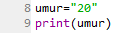
\includegraphics[scale=2]{figures/chapter 2/1.PNG}
    \end{center}

    \item String
    \begin{center}
        \centering
        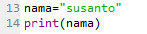
\includegraphics[scale=2]{figures/chapter 2/2.PNG}
    \end{center}

    \item Float
    \begin{center}
        \centering
        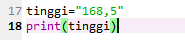
\includegraphics[scale=2]{figures/chapter 2/3.PNG}
    \end{center}

    
    \item outputnya
    \begin{center}
        \centering
        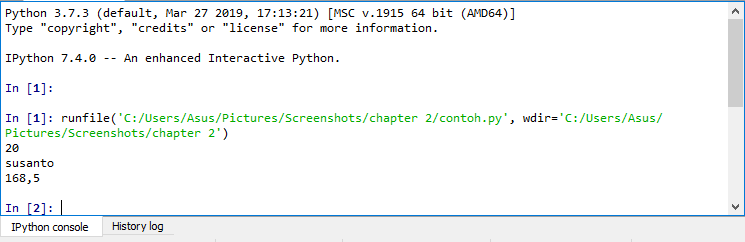
\includegraphics[scale=0.5]{figures/chapter 2/4.PNG}
    \end{center}
    \end{enumerate}



\item
tuliskan bagaimana kode untuk meminta input dari user dan tuliskan bagaimana melakukan output ke layar
\par\textbf{Jawaban}
Pyhton menggunakan kode () untuk mengambil input atau output contoh :
\begin{enumerate}
    \item Integer
    \begin{center}
        \centering
        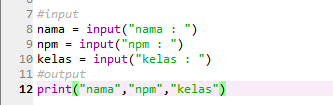
\includegraphics[scale=1.5]{figures/chapter 2/5.PNG}
    \end{center}

    \item String
    \begin{center}
        \centering
        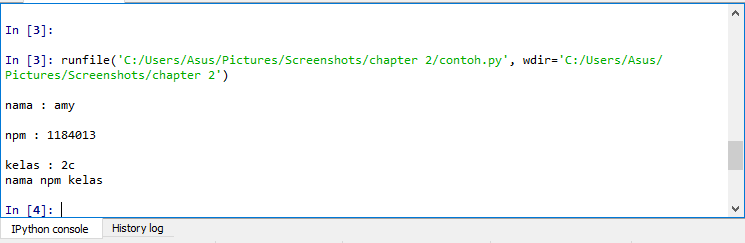
\includegraphics[scale=0.5]{figures/chapter 2/6.PNG}
    \end{center}
    \end{enumerate}

\item
Tuliskan operator dasar aritmatika, tambah, kali, kurang bagi, dan 
bagaimana mengubah string ke integer dan integer ke string.
\par\textbf{Jawaban}Contohnya dalam penggunaan aritmatika
\begin{enumerate}
    \item kodingan
    \begin{center}
        \centering
        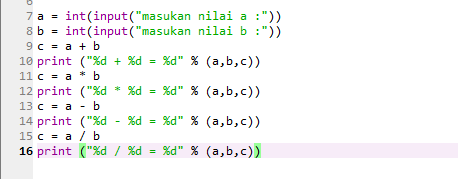
\includegraphics[scale=1]{figures/chapter 2/7.PNG}
    \end{center}
    
        \item hasil
    \begin{center}
        \centering
        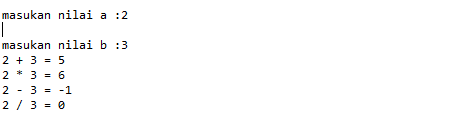
\includegraphics[scale=1.5]{figures/chapter 2/8.PNG}
    \end{center}
    
            \item cara merubah string ke intiger dan integer ke string
    \begin{center}
        \centering
        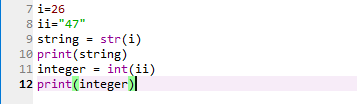
\includegraphics[scale=1.5]{figures/chapter 2/9.PNG}
    \end{center}
\end{enumerate}
\item
Tuliskan dan jelaskan sintak untuk perulangan, jenis-jenisnya contoh kode dan cara pakainya di python
\par\textbf{Jawaban}perulangan adalah sebuah perintah untuk memerintahkan untuk run sesuai yang diinginkan, ada 2 yaitu for dan while contoh :
\begin{enumerate}
    \item for
    \begin{center}
        \centering
        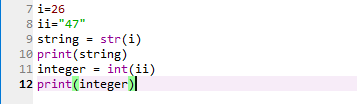
\includegraphics[scale=1]{figures/chapter 2/10.PNG}
    \end{center}
    
        \item while
    \begin{center}
        \centering
        \includegraphics[scale=1]{figures/chapter 2/.PNG}
    \end{center}
    \end{enumerate}
\item
Tuliskan jelaskan cara pakai sintak untuk memilih kondisi, dan bagiamana contoh sintak kondisi di dalam kondisi.
\par\textbf{Jawaban} Ada 3 kondisi yaitu if,ifelse dan ifelifelse
\begin{enumerate}
    \item if
    \begin{center}
        \centering
        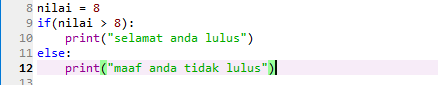
\includegraphics[scale=1]{figures/chapter 2/11.PNG}
    \end{center}
    
        \item ifelse
    \begin{center}
        \centering
        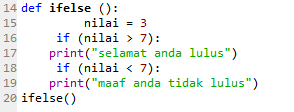
\includegraphics[scale=1.5]{figures/chapter 2/12.PNG}
    \end{center}
    
            \item ifelifelse
    \begin{center}
        \centering
        \includegraphics[scale=1.5]{figures/chapter 2/}
    \end{center}
\end{enumerate}
\item
Tuliskan apa saja jenis error yang sering ditemui di python dalam mengerjakan sintak diatas dan bagaimana cara mengatasinya.
\par\textbf{Jawaban} Error dapat terjadi karena kesalahan si pengetik atau typo dan dapat diperbaiki dengan cara try except bisa juga dilihat dari console
\item
Tuliskan dan jelaskan cara memakai Try Except.
\par\textbf{Jawaban} try except biasa digunakan dalam penanganan error di database,penggunaan IO dan lain-lain.

    \begin{center}
        \centering
        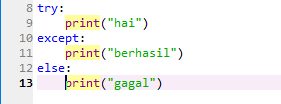
\includegraphics[scale=1.5]{figures/chapter 2/13.PNG}
    \end{center}

\end{enumerate}

\section{Ketrampilan Pemrograman}
Buat program di python dengan ketentuan:
\begin{enumerate}
\item
Buatlah luaran huruf yang dirangkai dari tanda bintang, pagar atau plus dari NPM kita.
Tanda bintang untuk NPM mod 3=0, tanda pagar untuk NPM mod 3 =1, tanda plus untuk NPM mod3=2.
Contoh Output : 
\begin{verbatim}
*****    *** ******     *****    ****
*******  *** ***  **    *** **  *****
***  ******* ******     ***  **** ***
***    ***** ***        ***       ***
***     **** ***        ***       ***
\end{verbatim}
NPM sesuai dengan nomor NPM nya.
\par\textbf{Jawaban}
    \begin{center}
        \centering
        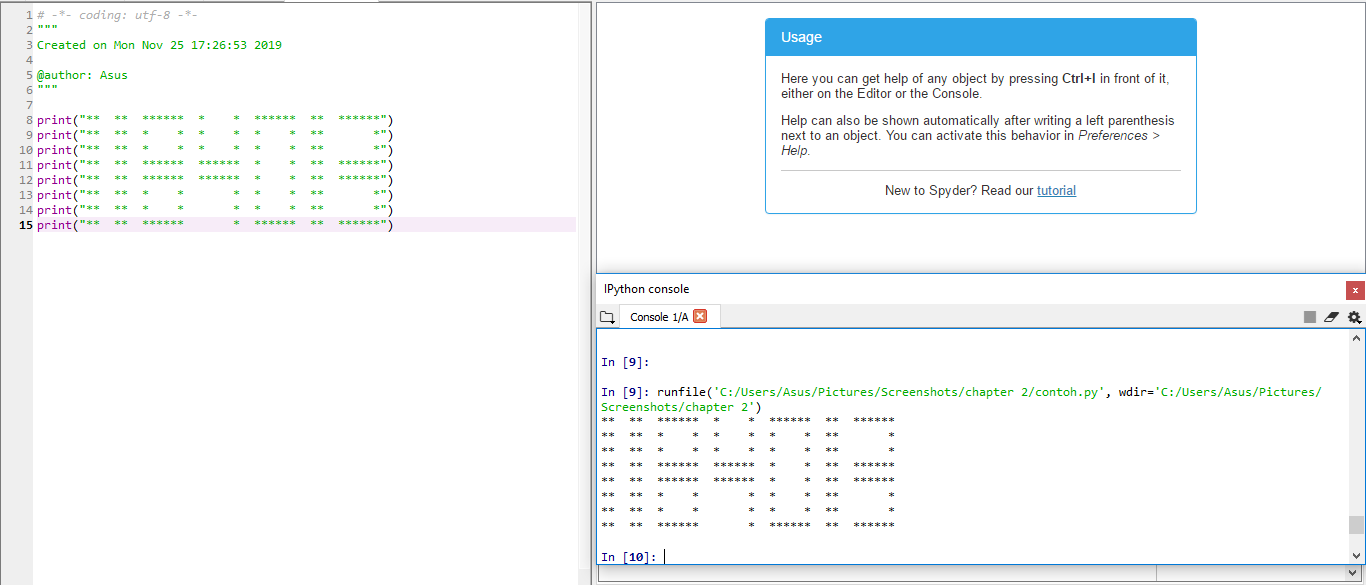
\includegraphics[scale=0.5]{figures/chapter 2/14.PNG}
    \end{center}
\item
Buatlah program hello word dengan input NPM yang disimpan dalam sebuah variabel string bernama \textbf{NPM} dan output sebanyak dua dijit belakang NPM, 
contoh NPM : 113040087 maka akan ada output sebanyak 87 dengan tulisan `Hallo, 113040087 apa kabar?'
\begin{verbatim}
Input : 113040087
Output : 
Halo, 113040087 apa kabar? 
Halo, 113040087 apa kabar?
Halo, 113040087 apa kabar?
Halo, 113040087 apa kabar?
Halo, 113040087 apa kabar?
Halo, 113040087 apa kabar?
Halo, 113040087 apa kabar?
Halo, 113040087 apa kabar?
.....87 kali...
\end{verbatim}
\par\textbf{Jawaban} 
    \begin{center}
        \centering
        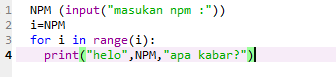
\includegraphics[scale=1.5]{figures/chapter 2/15.PNG}
    \end{center}
\item
Buatlah program hello word dengan input nama yang disimpan dalam sebuah variabel string bernama \textbf{NPM} dan beri luaran output berupa tiga karakter belakang dari NPM sebanyak penjumlahan tiga dijit tersebut, 
\begin{verbatim}
Input : 113040087
Output : Halo, Nama apa kabar? 
Halo, 087 apa kabar?
Halo, 087 apa kabar?
Halo, 087 apa kabar?
Halo, 087 apa kabar?
Halo, 087 apa kabar?
Halo, 087 apa kabar?
Halo, 087 apa kabar?
........15 kali(0+8+7).........
\end{verbatim}
\item
Buatlah program hello word dengan input nama yang disimpan dalam sebuah variabel string bernama \textbf{NPM} dan beri luaran output berupa digit ketiga dari belakang dari variabel NPM, 
\begin{verbatim}
Input : 113040087
Output :
Halo, 0 apa kabar?
\end{verbatim}
\par\textbf{Jawaban}
\par\textbf{Jawaban} 
    \begin{center}
        \centering
        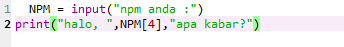
\includegraphics[scale=1.5]{figures/chapter 2/16.PNG}
    \end{center}
\item
\label{digitvar}
(untuk soal no \ref{digitvar} dan selanjutnya wajib menggunakan perulangan dan kondisi) buat program dengan mengisi variabel alfabet dengan nomor npm satu persatu berurut.
Contoh untuk NPM : 113040087 maka,
\begin{verbatim}
a = 1
b = 1
c = 3
e = 0
f = 4
g = 0
h = 0
i = 8
j = 7
\end{verbatim}
Lakukan print NPM lengkap anda menggunakan variabel diatas :
\par\textbf{Jawaban}
    \begin{center}
        \centering
        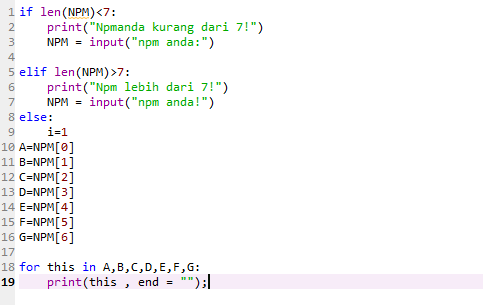
\includegraphics[scale=1.5]{figures/chapter 2/17.PNG}
    \end{center}
contoh : 113040087
\item
Dari soal no \ref{digitvar}, Lakukan penjumlahan dari seluruh variabel tersebut,
\par\textbf{Jawaban}
    \begin{center}
        \centering
        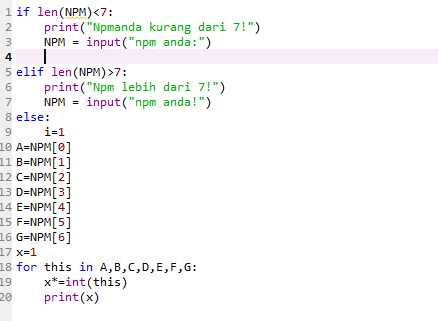
\includegraphics[scale=1.5]{figures/chapter 2/18.PNG}
    \end{center}
\item 
Dari soal no \ref{digitvar}, Lakukan perkalian dari seluruh variabel tersebut,
\par\textbf{Jawaban}
    \begin{center}
        \centering
        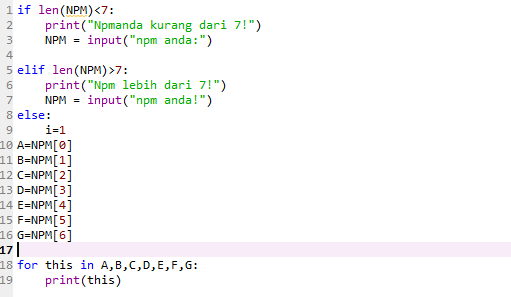
\includegraphics[scale=1.5]{figures/chapter 2/19.PNG}
    \end{center}
\item
Dari soal no \ref{digitvar}, Lakukan print secara vertikal dari NPM anda menggunakan variabel diatas. Contoh:
\begin{verbatim}
1
1
3
0
4
0
0
8
7
\end{verbatim}
\par\textbf{Jawaban}
    \begin{center}
        \centering
        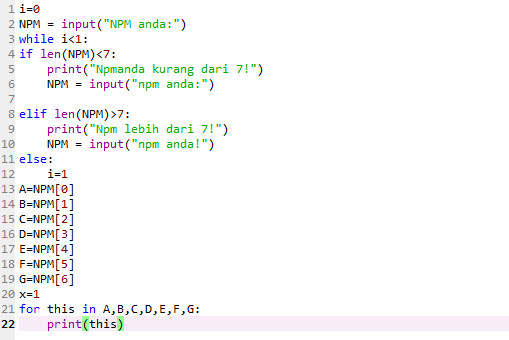
\includegraphics[scale=1.5]{figures/chapter 2/20.PNG}
    \end{center}
\item
Dari soal no \ref{digitvar}, Lakukan print NPM anda tapi hanya dijit genap saja. Contoh:
\begin{verbatim}
48
\end{verbatim}
\par\textbf{Jawaban} 
    \begin{center}
        \centering
        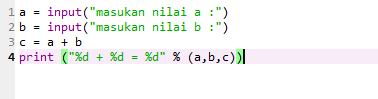
\includegraphics[scale=1.5]{figures/chapter 2/21.PNG}
    \end{center}

\item
Dari soal no \ref{digitvar}, Lakukan print NPM anda tapi hanya dijit ganjil saja. Contoh:
\begin{verbatim}
1137
\end{verbatim}
    \begin{center}
        \centering
        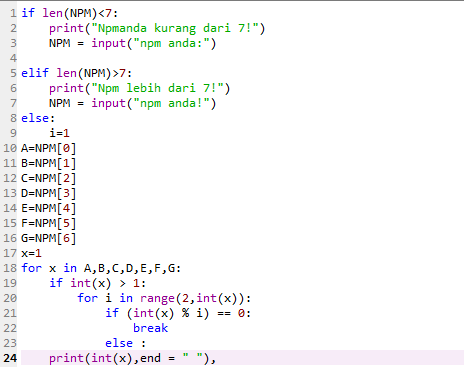
\includegraphics[scale=0.7]{figures/chapter 2/22.PNG}
    \end{center}
\item 
Dari soal no \ref{digitvar}, Lakukan print NPM anda tapi hanya dijit yang termasuk bilangan prima saja. Contoh:
\begin{verbatim}
37
\end{verbatim}
\end{enumerate}


\section{Ketrampilan Penanganan Error}
Bagian Penanganan error dari script python.
\begin{enumerate}
\item
Tuliskan peringatan error yang didapat dari mengerjakan praktek kedua ini, dan jelaskan cara penanganan error tersebut.
\par\textbf{Jawaban} berikut adalah contoh error karena data yang harusnya integer malah string dan cara penanganannya menggunakan try except
    \begin{center}
        \centering
        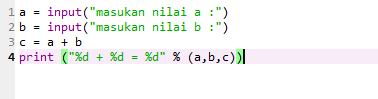
\includegraphics[scale=0.7]{figures/chapter 2/21.PNG}
    \end{center}

    \begin{center}
        \centering
        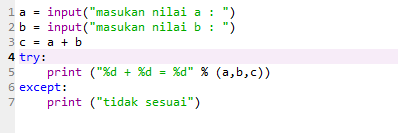
\includegraphics[scale=0.7]{figures/chapter 2/23.PNG}
    \end{center}
\item
Membuat file 2err.py dan mengisinya dengan script pengisian variabel sebagai string dan pengisian variabel sebagai interger. 
Kemudian jumlahkan antara variabel integer dan string dan tangkap jenis errornya, gunakan try except untuk menunjukkan error tersebut dengan
bahasa indonesia.
\par\textbf{Jawaban}
    \begin{center}
        \centering
        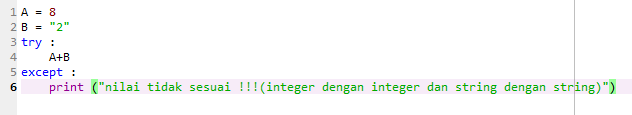
\includegraphics[scale=0.7]{figures/chapter 2/24.PNG}
    \end{center}

    \begin{center}
        \centering
        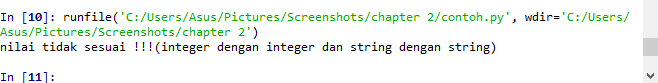
\includegraphics[scale=0.7]{figures/chapter 2/25.PNG}
    \end{center}
\end{enumerate}



